\hypertarget{visualisation-de-la-donnuxe9e}{%
\section{Visualisation de la
donnée}\label{visualisation-de-la-donnuxe9e}}

Pour rappel, le TD d'introduction sur la collecte de données est en
ligne à cette adresse :
\url{https://github.com/lennepkade/1A_DATA-COLLECT}

Petit rappel de l'introduction du TD précédent : le SIG est outil qui
permet aussi de réaliser des cartes. Pour ce faire, deux modes de
représentation des données sont utilisés par ces logiciels :

\begin{itemize}
\tightlist
\item
  Mode \textbf{vecteur} (représentation objet fondée sur des points,
  lignes, polygones)
\item
  Mode \textbf{raster} ou \textbf{image} (représentation matricielle
  avec partition complète de l'espace)
\end{itemize}

\begin{figure}
\centering
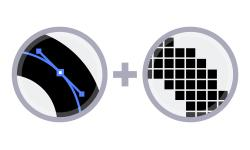
\includegraphics{figures/icon_vector-raster.jpg}
\caption{Différence entre vecteur (à gauche) et raster (à droite)}
\end{figure}

Ces données ont obligatoirement :

\begin{enumerate}
\def\labelenumi{\arabic{enumi}.}
\tightlist
\item
  un système de coordonnées :

  \begin{itemize}
  \tightlist
  \item
    il peut s'agir d'un système de coordonnées projetées (ex. Lambert-93
    ou code EPSG:2154 pour la France, liée au système géodésique RGF-93)
  \item
    il peut s'agir d'un système de coordonnées géographiques (ex. WGS-84
    ou code EPSG:4326 pour le monde)
  \end{itemize}
\item
  des coordonnées issues du système précédent (en lat/long ou en mètres)
\end{enumerate}

L'objectif de ce TD est de vous faire produire des cartes en respectant
la sémiologie graphique, c'est-à-dire les règles graphiques à respecter
pour bien représenter votre donnée.

\hypertarget{les-grands-types-de-donnuxe9es-uxe0-repruxe9senter}{%
\subsection{Les grands types de données à
représenter}\label{les-grands-types-de-donnuxe9es-uxe0-repruxe9senter}}

\begin{itemize}
\tightlist
\item
  Une information quantitative mais de surface variable (ex : nombre
  d'habitants par ville) :
  \href{https://www.geoclip.fr/portfolio-item/carte-a-symboles-proportionnels/}{symbole
  proportionnel} :
\end{itemize}

\begin{figure}
\centering
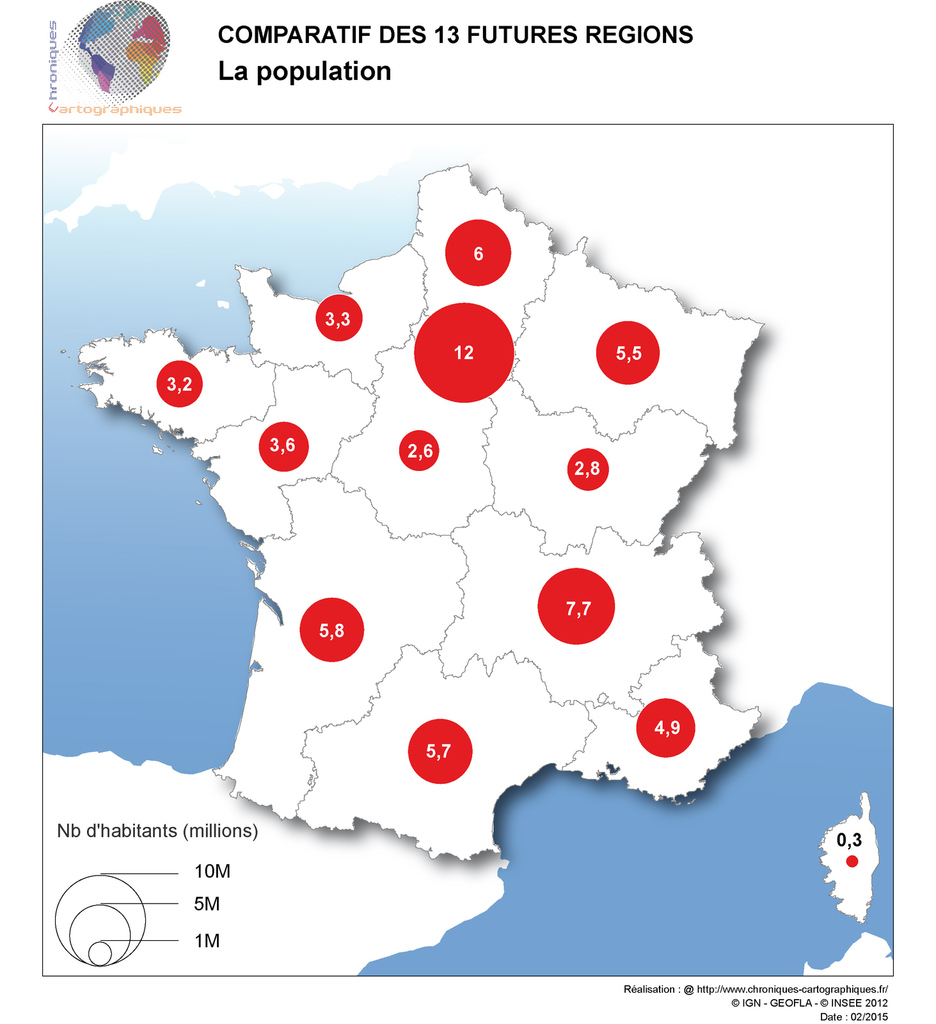
\includegraphics{figures/example_proportion.jpg}
\caption{Représenter une information quantitative de surface variable}
\end{figure}

\begin{itemize}
\tightlist
\item
  Une information quantitative mais relative à la surface (ex : nombre
  d'habitants par km/2) :
  \href{https://fr.wikipedia.org/wiki/Carte_choropl\%C3\%A8the}{carte
  choroplèthe} ou une densité de motifs (traits de plus en plus fins par
  exemple) :
\end{itemize}

\begin{figure}
\centering
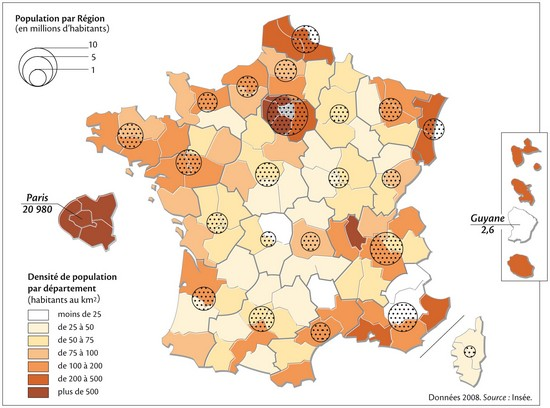
\includegraphics{figures/example_proportion_and_cho.jpg}
\caption{Combinaison de symboles proportionnels avec un dégradé de
couleurs pour les informations quantitatives relatives à la surface}
\end{figure}

\begin{itemize}
\tightlist
\item
  Une information qualitative sur une surface : des couleurs ou des
  motifs différents :
\end{itemize}

\begin{figure}
\centering
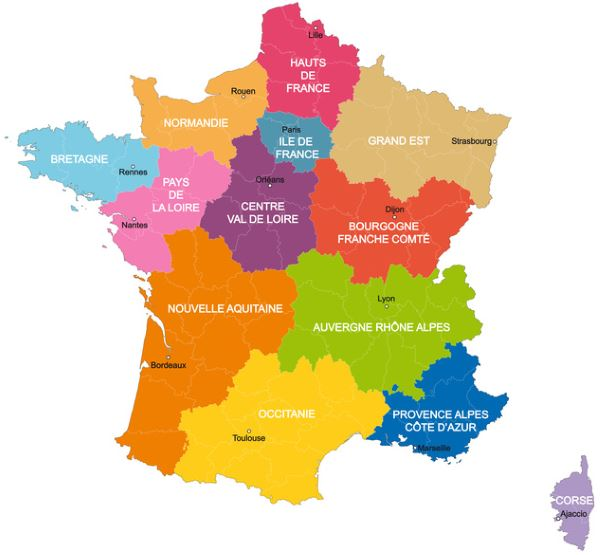
\includegraphics{figures/examples_regions.jpg}
\caption{Différentes régions de la France}
\end{figure}

Une information qualitative sur un point : un symbôle/icône. :

\begin{figure}
\centering
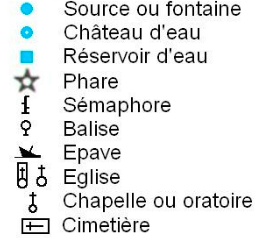
\includegraphics{figures/examples_ponctuel_ign.png}
\caption{Aperçu de la sémiologie ponctuelle de la carte de l'IGN}
\end{figure}

\hypertarget{cruxe9er-un-nouveau-projet-qgis}{%
\section{Créer un nouveau projet
QGIS}\label{cruxe9er-un-nouveau-projet-qgis}}

Quand vous lancez QGIS, commencez par créer un nouveau projet :
\texttt{Projet\ \textgreater{}\ Nouveau}.

\hypertarget{choisir-une-projection-adaptuxe9e}{%
\subsection{Choisir une projection
adaptée}\label{choisir-une-projection-adaptuxe9e}}

Par défaut votre projet utilise le système de référence mondial WGS-84
(celui du GPS), nom de code EPSG:4326. Dans QGIS, le système de
référence du projet est toujours affiché en bas à droite de la fenêtre
de QGIS. Vous pouvez donc vérifier votre projection :

\begin{figure}
\centering
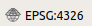
\includegraphics{figures/EPSG4326.png}
\caption{SCR actuel dans QGIS : EPSG:4326}
\end{figure}

Pour regarder les propriétés de votre projet :
\texttt{Projet\ \textgreater{}\ Propriétés}.

Dans l'onglet \texttt{SCR} (Système de Coordonnées de Référence),
recherchez \texttt{2154}, soit le code EPSG de la projection Lambert-93
qui est la projection officielle en France depuis 2000 et obligatoire
pour les données publiques.

Si vous voulez en savoir plus sur cette projection, reportez-vous à la
\href{https://fr.wikipedia.org/wiki/Projection_conique_conforme_de_Lambert}{page
Wikipedia} dédiée.

Une fois la projection Lambert-93 (EPSG:2154) validée, vous pouvez à
nouveau vérifier en bas à droite de la fenêtre de QGIS :

\begin{figure}
\centering
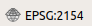
\includegraphics{figures/EPSG2154.png}
\caption{SCR actuel dans QGIS : EPSG:2154}
\end{figure}

Dans l'onglet \texttt{Général}, pensez à donner un nom à votre projet,
il apparaîtra à côté du nom de la fenêtre QGIS.

Une fois ces manipulations effectuées, vous pouvez sauvegarder votre
projet dans votre dossier de travail (ce dossier contiendra également
par la suite vos données vecteur/raster).
\texttt{Projet\ \textgreater{}\ Enregistrer\ sous...}

\hypertarget{charger-les-donnuxe9es}{%
\subsection{Charger les données}\label{charger-les-donnuxe9es}}

Pour ce TD, il est fourni un fichier vectoriel de type polygone où sont
numérisées 10 parcelles de l'exploitation de Borret :
\texttt{parcelles\_borret.gpkg}.

En plus des parcelles, 2 fichiers de type \texttt{csv} vous sont fournis
:

\begin{itemize}
\tightlist
\item
  \texttt{assolement\_2018.csv}, la liste par parcelle de ce qui a été
  récolté en 2018
\item
  \texttt{production.csv}, la production (qt/ha) par type de culture
\end{itemize}

\hypertarget{repruxe9senter-les-parcelles}{%
\section{Représenter les parcelles}\label{repruxe9senter-les-parcelles}}

Dans QGIS 3, il n'y a plus qu'un bouton unique pour ouvrir n'importe
quel type de couche.

\begin{figure}
\centering
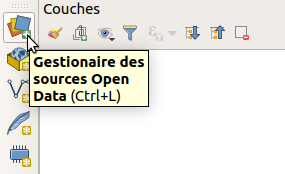
\includegraphics[width=\textwidth,height=1.5625in]{figures/QGIS_charger.png}
\caption{Charger une couche dans QGIS}
\end{figure}

Une fois le fichier \texttt{parcelles\_borret.gpkg} ouvert, vous pouvez
regarder ce qu'il contient en ouvrant sa table d'attributs
(\texttt{clic\ droit\ sur\ la\ couche\ \textgreater{}\ ouvrir\ la\ table\ d\textquotesingle{}attributs}).

Nous pouvons donc représenter pour l'instant uniquement les informations
contenues dans la table, donc soit le champs \texttt{fid}, soit le
champs \texttt{id\_parcelle}.

\hypertarget{couleur-et-uxe9tiquette-unique-par-parcelle}{%
\subsection{Couleur et étiquette unique par
parcelle}\label{couleur-et-uxe9tiquette-unique-par-parcelle}}

Il s'agit de représenter une information qualitative, donc chaque
parcelle aura sa propre couleur.

\hypertarget{uxe9tiquette}{%
\subsubsection{Étiquette}\label{uxe9tiquette}}

Clic droit \textgreater{} Propriété de la couche \textgreater{}
Étiquettes

\begin{figure}
\centering
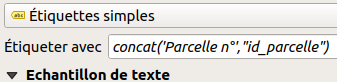
\includegraphics[width=\textwidth,height=1.04167in]{figures/etiquette_parcelle.png}
\caption{Étiquetter les parcelles}
\end{figure}

Dans étiquettes simples, choisissez le champs content l'identifiant de
la parcelle. N'hésitez pas à changer la police, à ajouter un ombre pour
mieux voir la police par exemple.

Si vous voulez ajouter en plus du numéro de la parcelle, un texte qui
indique `Parcelle n', il vous faut alors \textbf{concatener} deux textes
comme suit :

\texttt{concat(\textquotesingle{}Parcelle\ n\textquotesingle{},"id\_parcelle")}

Attention à bien mettre des guillemets simples pour ajouter du texte,
les double guillemets (") sont utilisés pour nommer les champs (comme
ici le champs \texttt{id\_parcelle}).

\begin{figure}
\centering
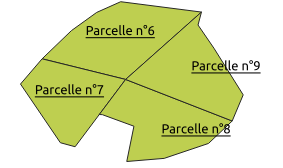
\includegraphics[width=\textwidth,height=1.5625in]{figures/parcelle_num.png}
\caption{Résultat de l'étiquettage}
\end{figure}

\hypertarget{couleur-symbologie}{%
\subsubsection{Couleur (symbologie)}\label{couleur-symbologie}}

\begin{figure}
\centering
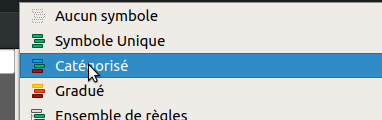
\includegraphics[width=\textwidth,height=1.5625in]{figures/symbologie.png}
\caption{Liste des symbologies}
\end{figure}

Dans l'onglet symbologie, sélectionner dans la liste Catégorisé.

La colonne servant coloriser les parcelles à est la même que pour les
étiquettes.

Ensuite la ligne \texttt{symbole} vous permet de modifier comment votre
polygone est représenté (style et largeur du contour de votre polygone
par exemple).

Puis vous pouvez choisir une palette de couleurs. Comme nous sommes sur
une information qualitative, nous prendrons que des couleurs
sélectionnées aléatoirement.

Le rendu est le suivant :

\begin{figure}
\centering
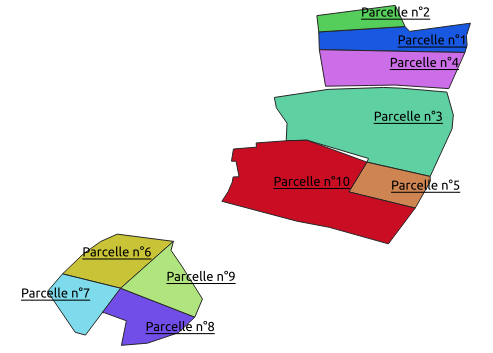
\includegraphics{figures/parcelles_categorise.png}
\caption{Liste des symbologies}
\end{figure}

\hypertarget{amuxe9lioration-de-la-carte}{%
\subsubsection{Amélioration de la
carte}\label{amuxe9lioration-de-la-carte}}

Pour améliorer la beauté de votre carte, vous pouvez par exemple :

\begin{itemize}
\tightlist
\item
  ajouter de la transparence à la couleur de chaque parcelle,
\item
  changer le ligne de contour du polygone,
\item
  changer de police.
\item
  choisir l'endoirt où sera placé votre texte
  (\texttt{étiquette\ \textgreater{}\ position\ \textgreater{}\ décalé\ du\ centroïd}
  par exemple)
\end{itemize}

\begin{figure}
\centering
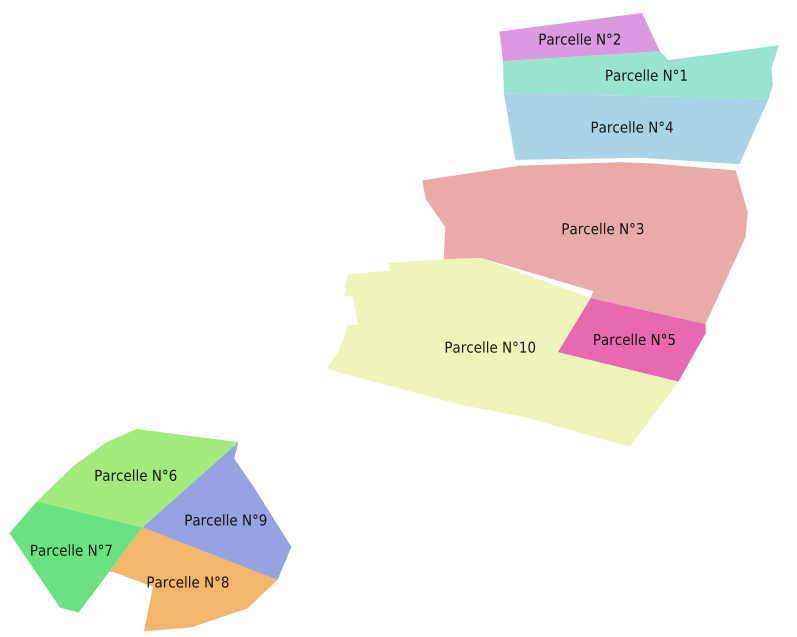
\includegraphics{figures/parcelle_style.png}
\caption{Affichage des parcelles amélioré}
\end{figure}

\hypertarget{cruxe9er-une-carte-exportable-jpgpdf}{%
\section{Créer une carte exportable
(jpg/pdf)}\label{cruxe9er-une-carte-exportable-jpgpdf}}

Une fois votre symbologie choisie, vous pouvez créer une mise en page
afin d'y ajouter des éléments essentiels de compréhension comme :

\begin{itemize}
\tightlist
\item
  un titre
\item
  une légende
\item
  le nord
\item
  la localisation sur un planisphère
\end{itemize}

Pour ce faire, aller dans le menu
\texttt{Projet\ \textgreater{}\ Nouvelle\ mise\ en\ page}.

Pour ajouter la carte que vous venez de réaliser dans Qgis, cliquez sur
l'icône \texttt{Ajouter\ une\ carte} dans le menu à gauche.

\begin{figure}
\centering
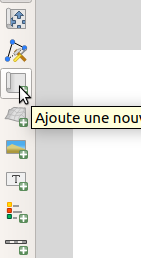
\includegraphics{figures/composer_addMap.png}
\caption{Ajouter une carte}
\end{figure}

Vous pouvez déplacer le contenu de la carte en utilisant l'icône avec
les flêches qui vont dans les 4 sens.

Enfin, si l'emprise de votre carte ne vous satisfait pas, le plus simple
est de retourner dans la fenêtre principal de Qgis puis : clic droit sur
les parcelles, et choisissez ``Zommer sur la couche''.

Puis dans le composeur, cliquer sur l'icône
\texttt{Set\ Map\ Extent\ to\ Match\ Main\ Canvas\ Extent} pour que
votre carte utilise la même emprise que l'emprise de la fenêtre
principale de QGIS.

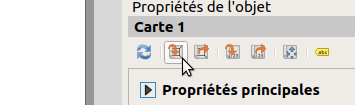
\includegraphics{figures/composer_mapExtent.png}.

Vous pouvez ajouter plusieurs textes : - un titre - les crédits (qui a
fait la carte et avec des données de quelles sources ?).

Et n'oubliez pas d'ajouter une légende (icône légende) et une flêche
nord (icône fléche nord).

Quand la carte vous convient, faites
\texttt{Mise\ en\ page\ \textgreater{}\ Exporter\ au\ format\ PDF},
\texttt{image} ou \texttt{SVG} selon l'utilisation voulue.

N'oubliez pas de sauvegarder votre projet qui contiendra désormais votre
première mise en page, félicitations !

\hypertarget{ajouter-lassolement-et-la-production-de-lannuxe9e-2018}{%
\section{Ajouter l'assolement et la production de l'année
2018}\label{ajouter-lassolement-et-la-production-de-lannuxe9e-2018}}

Gràce au fichier \texttt{assolement\_2018.csv}, nous savons quel type de
culture à été récolté pour chaque parcelle.

Grâce au fichier \texttt{production.csv}, nous connaissons la production
en quintaux/ha pour chaque type de culture.

Il faut donc désormais ajouter des colonnes à notre fichier
\texttt{parcelles.gpkg} pour pouvoir afficher les cultures, et la
production totale de la parcelle. Mais pas question de le faire en les
saisissant à la main !

Importer vos fichiers CSV directement dans QGIS à partir
(\texttt{Couche\ \textgreater{}\ Ajouter\ une\ couche\ \textgreater{}\ Ajouter\ une\ couche\ de\ texte\ délimité}).
Sélectionner votre fichier csv et cocher la case
\texttt{Détecter\ les\ types\ de\ champs} pour que QGIS traite bien les
nombres comme une colonne de type numérique et non textuelle. Ces
fichiers CSV n'ont pas de géométrie (pas de coordonnées X et Y, il
faudra donc aussi cocher \texttt{Pas\ de\ géométrie} dans la partie
\texttt{Définition\ de\ la\ géométrie}).

Pour regarder les informations contenues dans ces fichiers, vous pouvez
ouvrir leur table d'attributs comme pour toutes les couches de type
texte/vectoriel sur QGIS.

Pour lier des données entre elles, il nous faut un champs (colonne) en
commun, puis nous pouvons faire ce qu'on appelle une jointure à partir
de notre fichier parcelles :
\texttt{Clic\ droit\ \textgreater{}\ Propriété\ de\ la\ couche\ \textgreater{}\ Jointure}.

Une fois que vous avez trouver la colonne en commun entre le fichier
parcelle et le fichier csv, vous pouvez faire la jointure. Une fois
cette dernière faite, ouvrez la table attributaire du fichier
\texttt{parcelles} et vérifier qu'il contient bien une nouvelle colonne
bien remplie. Bravo, vous venez de faire votre première jointure :). Il
ne vous reste plus qu'à faire la deuxième désormais !

\hypertarget{sauvegarder-la-jointure}{%
\subsection{Sauvegarder la jointure}\label{sauvegarder-la-jointure}}

Les jointures sont en fait un lien entre votre fichier vectoriel et les
fichiers csv, c'est-à-dire que si quelqu'un modifie le fichier CSV, la
prochaine fois que vous utiliserez votre projet QGIS, vous aurez alors
une cartographie différente.

Pour sauvegarder et donc figer la jointure, vous pouvez faire un clic
droit sur votre couche, puis
\texttt{Exporter\ \textgreater{}\ Sauvegarder\ les\ entités\ sous...}.

\hypertarget{cartographier-la-production-uxe0-lhectare}{%
\subsection{Cartographier la production à
l'hectare}\label{cartographier-la-production-uxe0-lhectare}}

Réaliser une carte qui montre en étiquette le type de culture, et en
couleur (quantitatif) la production à l'hectare, c'est ce qu'on appelle
une carte choroplèthe.

\hypertarget{cartographier-la-production-totale-par-parcelle}{%
\subsection{Cartographier la production totale par
parcelle}\label{cartographier-la-production-totale-par-parcelle}}

L'objectif de cette partie est de réaliser qui montre la production
totale par parcelle.

Pour réaliser cette carte, il faut représenter la donnée d'une façon
moins conventionnelle, à partir de symbole proportionnel. Comme la
taille de la parcelle va impacter la production totale de la parcelle,
nous ne pouvons pas utiliser une carte choroplèthe comme à l'étape
précédente.

\hypertarget{calculer-la-production-uxe0-lhectare}{%
\subsubsection{Calculer la production à
l'hectare}\label{calculer-la-production-uxe0-lhectare}}

\begin{figure}
\centering
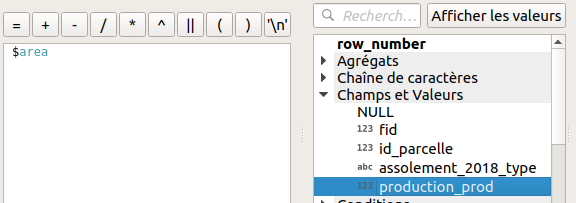
\includegraphics{figures/ajout_champ_production.png}
\caption{Cet outil facilite l'écriture d'expressions}
\end{figure}

Tout d'abord, nous connaissons la production à l'hectare selon le type
de culture. Il faut donc créer un nouveau champ nommé `production',
\texttt{Clic\ droit\ \textgreater{}\ ouvrir\ la\ table\ d\textquotesingle{}attributs}
puis :

\begin{itemize}
\tightlist
\item
  Ouvrir la calculatrice de champ (ctrl+i pour les geeks)
\item
  Cocher \texttt{Créer\ un\ nouveau\ champ}
\item
  Nom : `prod\_totale'
\item
  La formule à saisir est : \(area/10000 * "production_prod"\) . Mais
  attention, dans le cas présenté, la colonne contenant la production à
  l'hectare par type de culture s'appelle \emph{``production\_prod''},
  pensez à bien utiliser l'outil d'aide à la création d'expression pour
  retrouver le nom de votre colonne dans la partie
  \texttt{Champs\ et\ valeurs} (image ci-dessus)
\end{itemize}

\texttt{\$area} représente la surface du polygone selon l'unité de
mesure de la projection utilisée, comme nous utilisons du Lambert-93
(EPSG:2154), l'unité est le mètre. Donc pour calculer en hectare, nous
divisons par 10 000 la surface que nous multiplions aussi par la
production à l'hectare.

\hypertarget{guxe9nuxe9rer-le-centrouxefd-des-polygones}{%
\subsubsection{Générer le centroïd des
polygones}\label{guxe9nuxe9rer-le-centrouxefd-des-polygones}}

Une fois la colonne contenant la totalité de la production de la
parcelle a été calculée, nous pouvons générer les centroïds des
polygones, c'est-à-dire leur centre géographique.

Pour cela, dans la \texttt{boîte\ à\ outils\ de\ traitements},
rechercher le mot \texttt{centroïdes}, et générez-les (pensez à bien
enregister le fichier dans un endroit choisi avec un nom
compréhensible).

Vous pouvez afficher plusieurs informations dans une étiquette comme le
type d'assolement, sauter une ligne, et la production totale de la
parcelle, pour cela on va concatener plusieurs textes, dont un
\texttt{\textbackslash{}n} qui signifie un saut de ligne.

\hypertarget{afficher-le-type-et-la-production-en-uxe9tiquette}{%
\paragraph{Afficher le type et la production en
étiquette}\label{afficher-le-type-et-la-production-en-uxe9tiquette}}

Dans l'étiquette, saisir l'expression suivante :
\texttt{concat("assolement\_2018\_type",\textquotesingle{}\textbackslash{}n\textquotesingle{},\ "prod\_totale",\textquotesingle{}qt\textquotesingle{})}

Pour vous familiariser avec l'outil, vous pouvez remplacer la production
totale par la production à l'ha et afficher une étiquette sous la forme
: \texttt{Maïs\ :\ 89qt/ha}

\hypertarget{guxe9nuxe9rer-les-cercles-proportionnels}{%
\paragraph{Générer les cercles
proportionnels}\label{guxe9nuxe9rer-les-cercles-proportionnels}}

Cette étape permet de déterminer la taille d'un symbole en fonction de
la valeur d'un champ. Dans notre cas, nous voulons faire varier la
taille du cercle en fonction de la production totale de la parcelle.

\begin{figure}
\centering
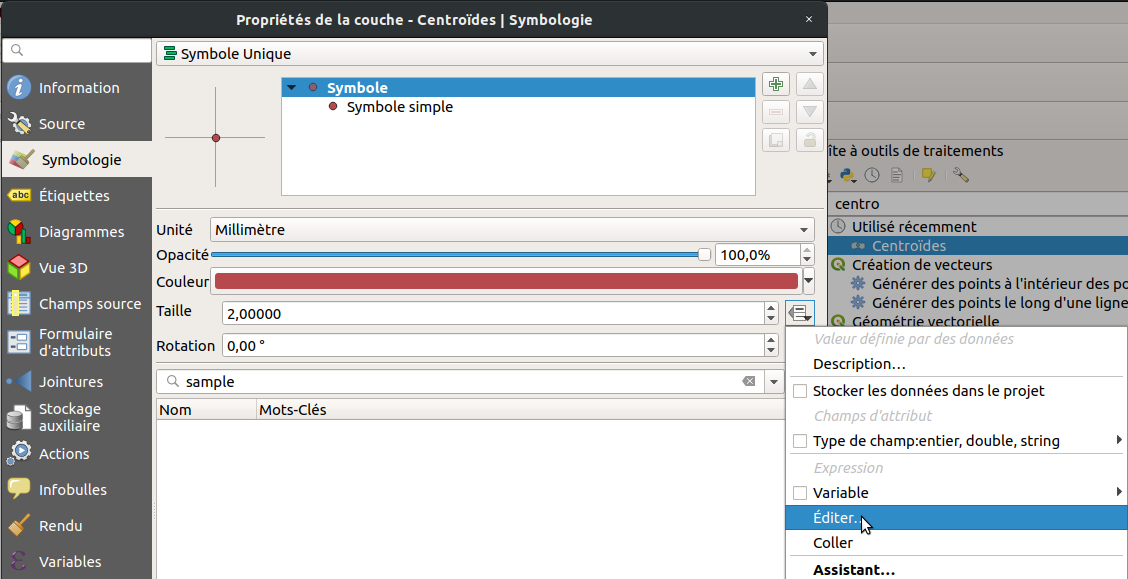
\includegraphics{figures/taille_fonction_champ.png}
\caption{Faire varier en taille en fonction d'une expression}
\end{figure}

Cependant, les valeurs allant d'environ 200 à plus de 1000 sont trop
importantes pour afficher dans une carte (que ce soit en cm ou en
pixels). Nous avons donc décidé de les diviser par 10 pour avoir des
nouvelles valeurs qui s'échelonnent entre 20 et 100. Pour cela, pas
besoin de créer un nouveau champ, il suffira de créer une simple
expression dans le calcul de la taille.

Dans la fenêtre du calcul d'expression quand vous éditer la taille du
cercle (fenêtre symbologie du centroide), vous retrouverez votre nom de
champ dans la partie \texttt{Champs\ et\ valeurs} comme montré
ci-dessous.

\begin{figure}
\centering
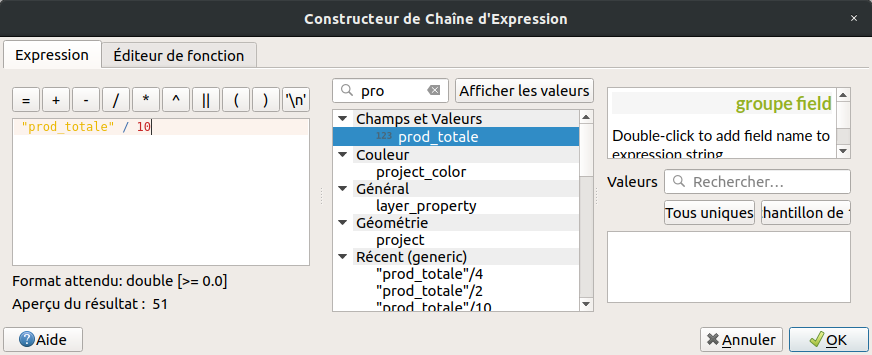
\includegraphics{figures/division_taille_champ.png}
\caption{Utiliser une expression pour calculer la taille du cercle}
\end{figure}

Choisissez le type \texttt{Point} comme unité de taille.

Maintenant, il faut générer la légende des cercles proportionnels. Pour
cela, toujours dans la partie symbologie, en bas à gauche cliquez sur
\texttt{Avancé\ \textgreater{}\ Légende\ définie\ par\ la\ taille\ des\ symboles}.

\begin{figure}
\centering
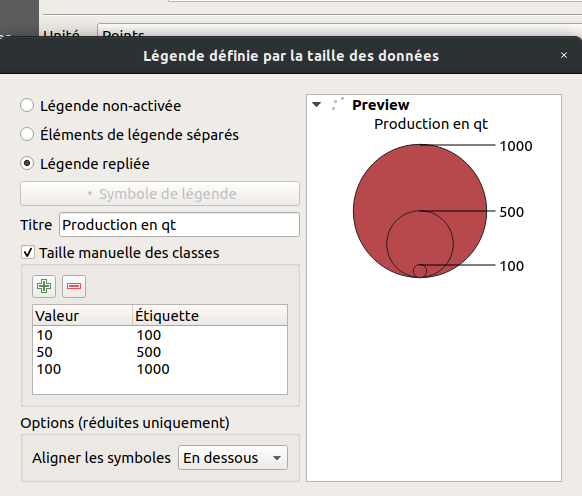
\includegraphics{figures/legend_propor.png}
\caption{Définissez votre légende proportionnelle}
\end{figure}

Pour légender les symboles proportionnels, on utilise ce qu'on appelle
une légende repliée. Il est nécessaire de définir la taille des classes
de manière manuelle car comme on a volontairement divisé par 10 la
taille des cercles. Il faura donc bien veiller à ce que la valeur du
cercle soit 10 fois inférieure à son étiquette.

\begin{figure}
\centering
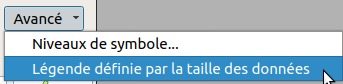
\includegraphics[width=\textwidth,height=0.52083in]{figures/legend_cercle.png}
\caption{Générer la légende des cercles proportionnels}
\end{figure}

Enfin, vous pouvez à nouveau faire une carte en combinant à la fois
l'information ponctuelle (ici la production totale de la parcelle) avec
la production à l'hectare selon le type de culture (exemple ci-dessous).

\begin{figure}
\centering
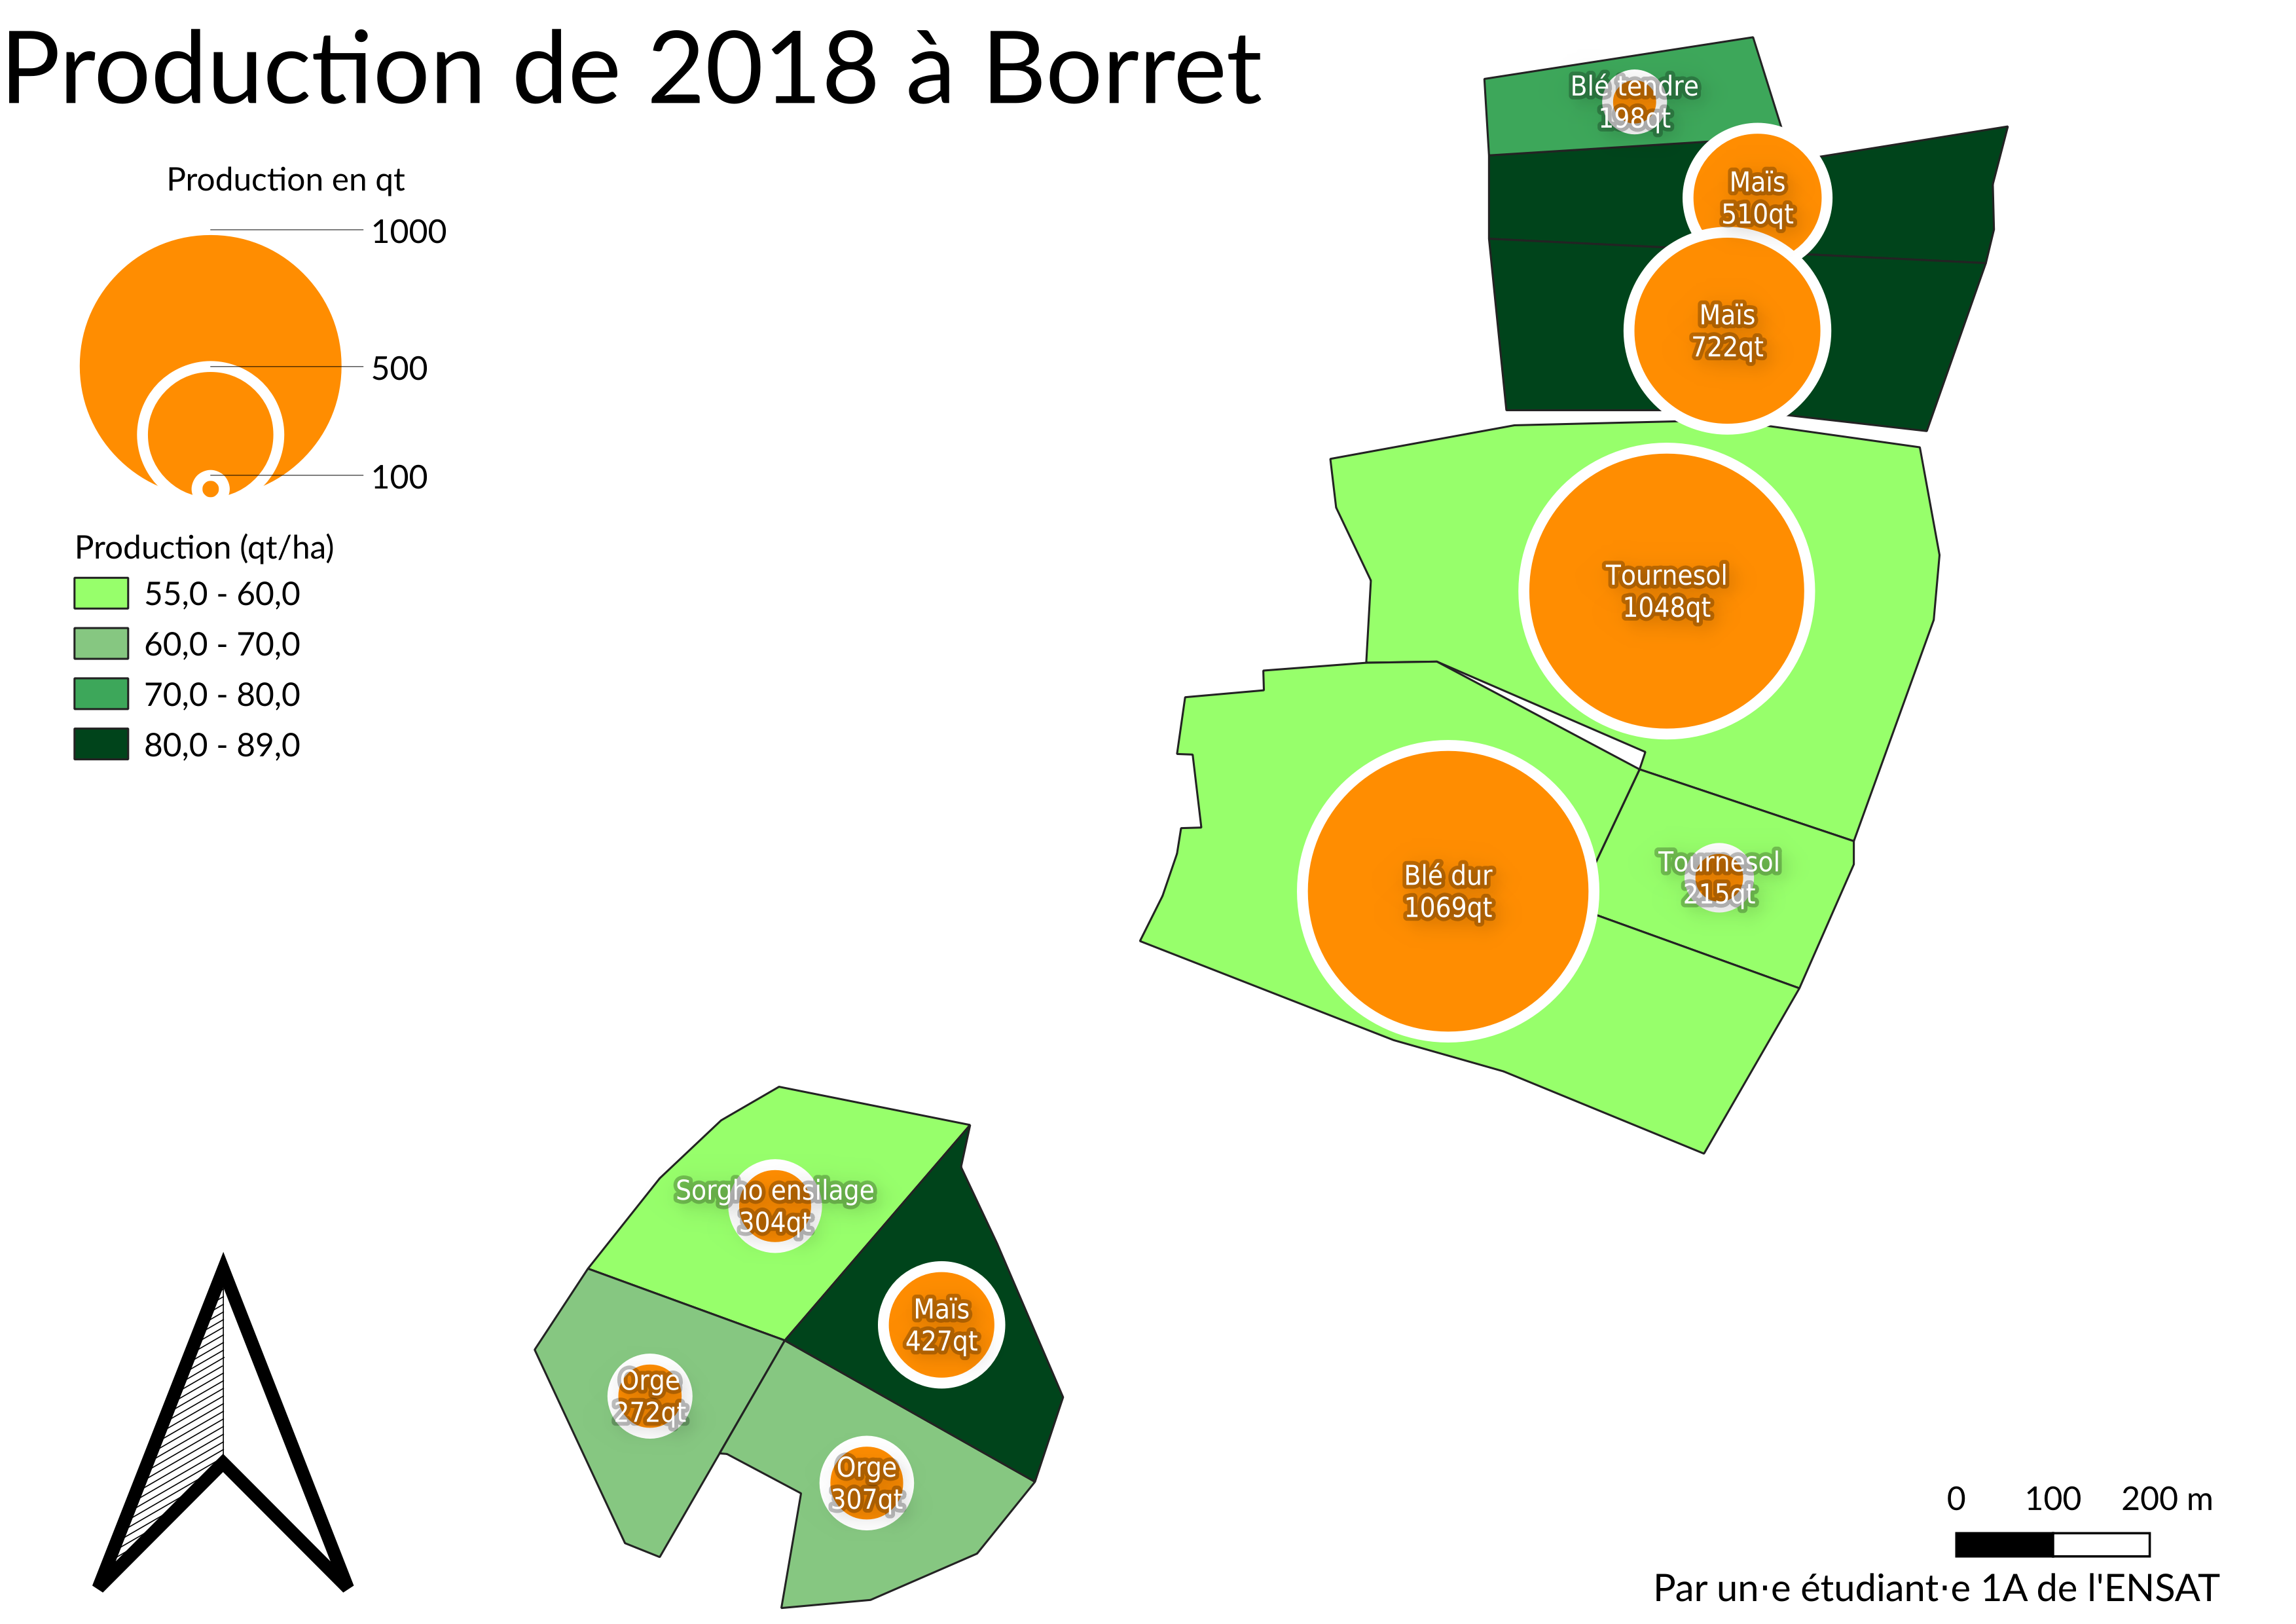
\includegraphics{figures/exemple_proportionnel.png}
\caption{Générer la légende des cercles proportionnels}
\end{figure}

N'hésitez pas à ajouter un fond de type OpenStreetMap.

\hypertarget{ajouter-une-carte-de-localisation-de-la-zone-duxe9tude}{%
\subsubsection{Ajouter une carte de localisation de la zone
d'étude}\label{ajouter-une-carte-de-localisation-de-la-zone-duxe9tude}}

Pour ajouter une petite carte servant à localiser la zone d'étude, il
faut tout d'abord cliquer comme pour votre première carte sur le bouton
\texttt{Ajouter\ une\ nouvelle\ carte\ à\ la\ mise\ en\ page}.

Sélectionner cette nouvelle carte, puis dans
\texttt{Propriétés\ de\ l\textquotesingle{}objet} , aller dans la partie
\texttt{Aperçu} et ajouter comme cadre votre première carte (celle
contenant vos parcelles).

Pour avoir un style différent de votre carte principale (celle des
parcelles) il faudra faire des allers-retours entre le composeur
d'impression et QGIS. Par exemple dans la fenêtre principale de QGIS,
mettez juste un fond de type OpenStreetMap par dessus l'ensemble des
couches (et désactivez les couches que vous ne voulez pas voir comme vos
parcelles), puis retourner dans le composeur pour
\texttt{Verrouiller\ les\ couches} de votre carte de localisation (dans
l'onglet \texttt{Propriétés\ de\ l\textquotesingle{}objet}). Ainsi que
vous remettrez dans le canvas principal de QGIS votre carte des
parcelles, l'aperçu de votre petite carte ne se mettra pas à jour à
gardera uniquement l'ancienne configuration.

\begin{figure}
\centering
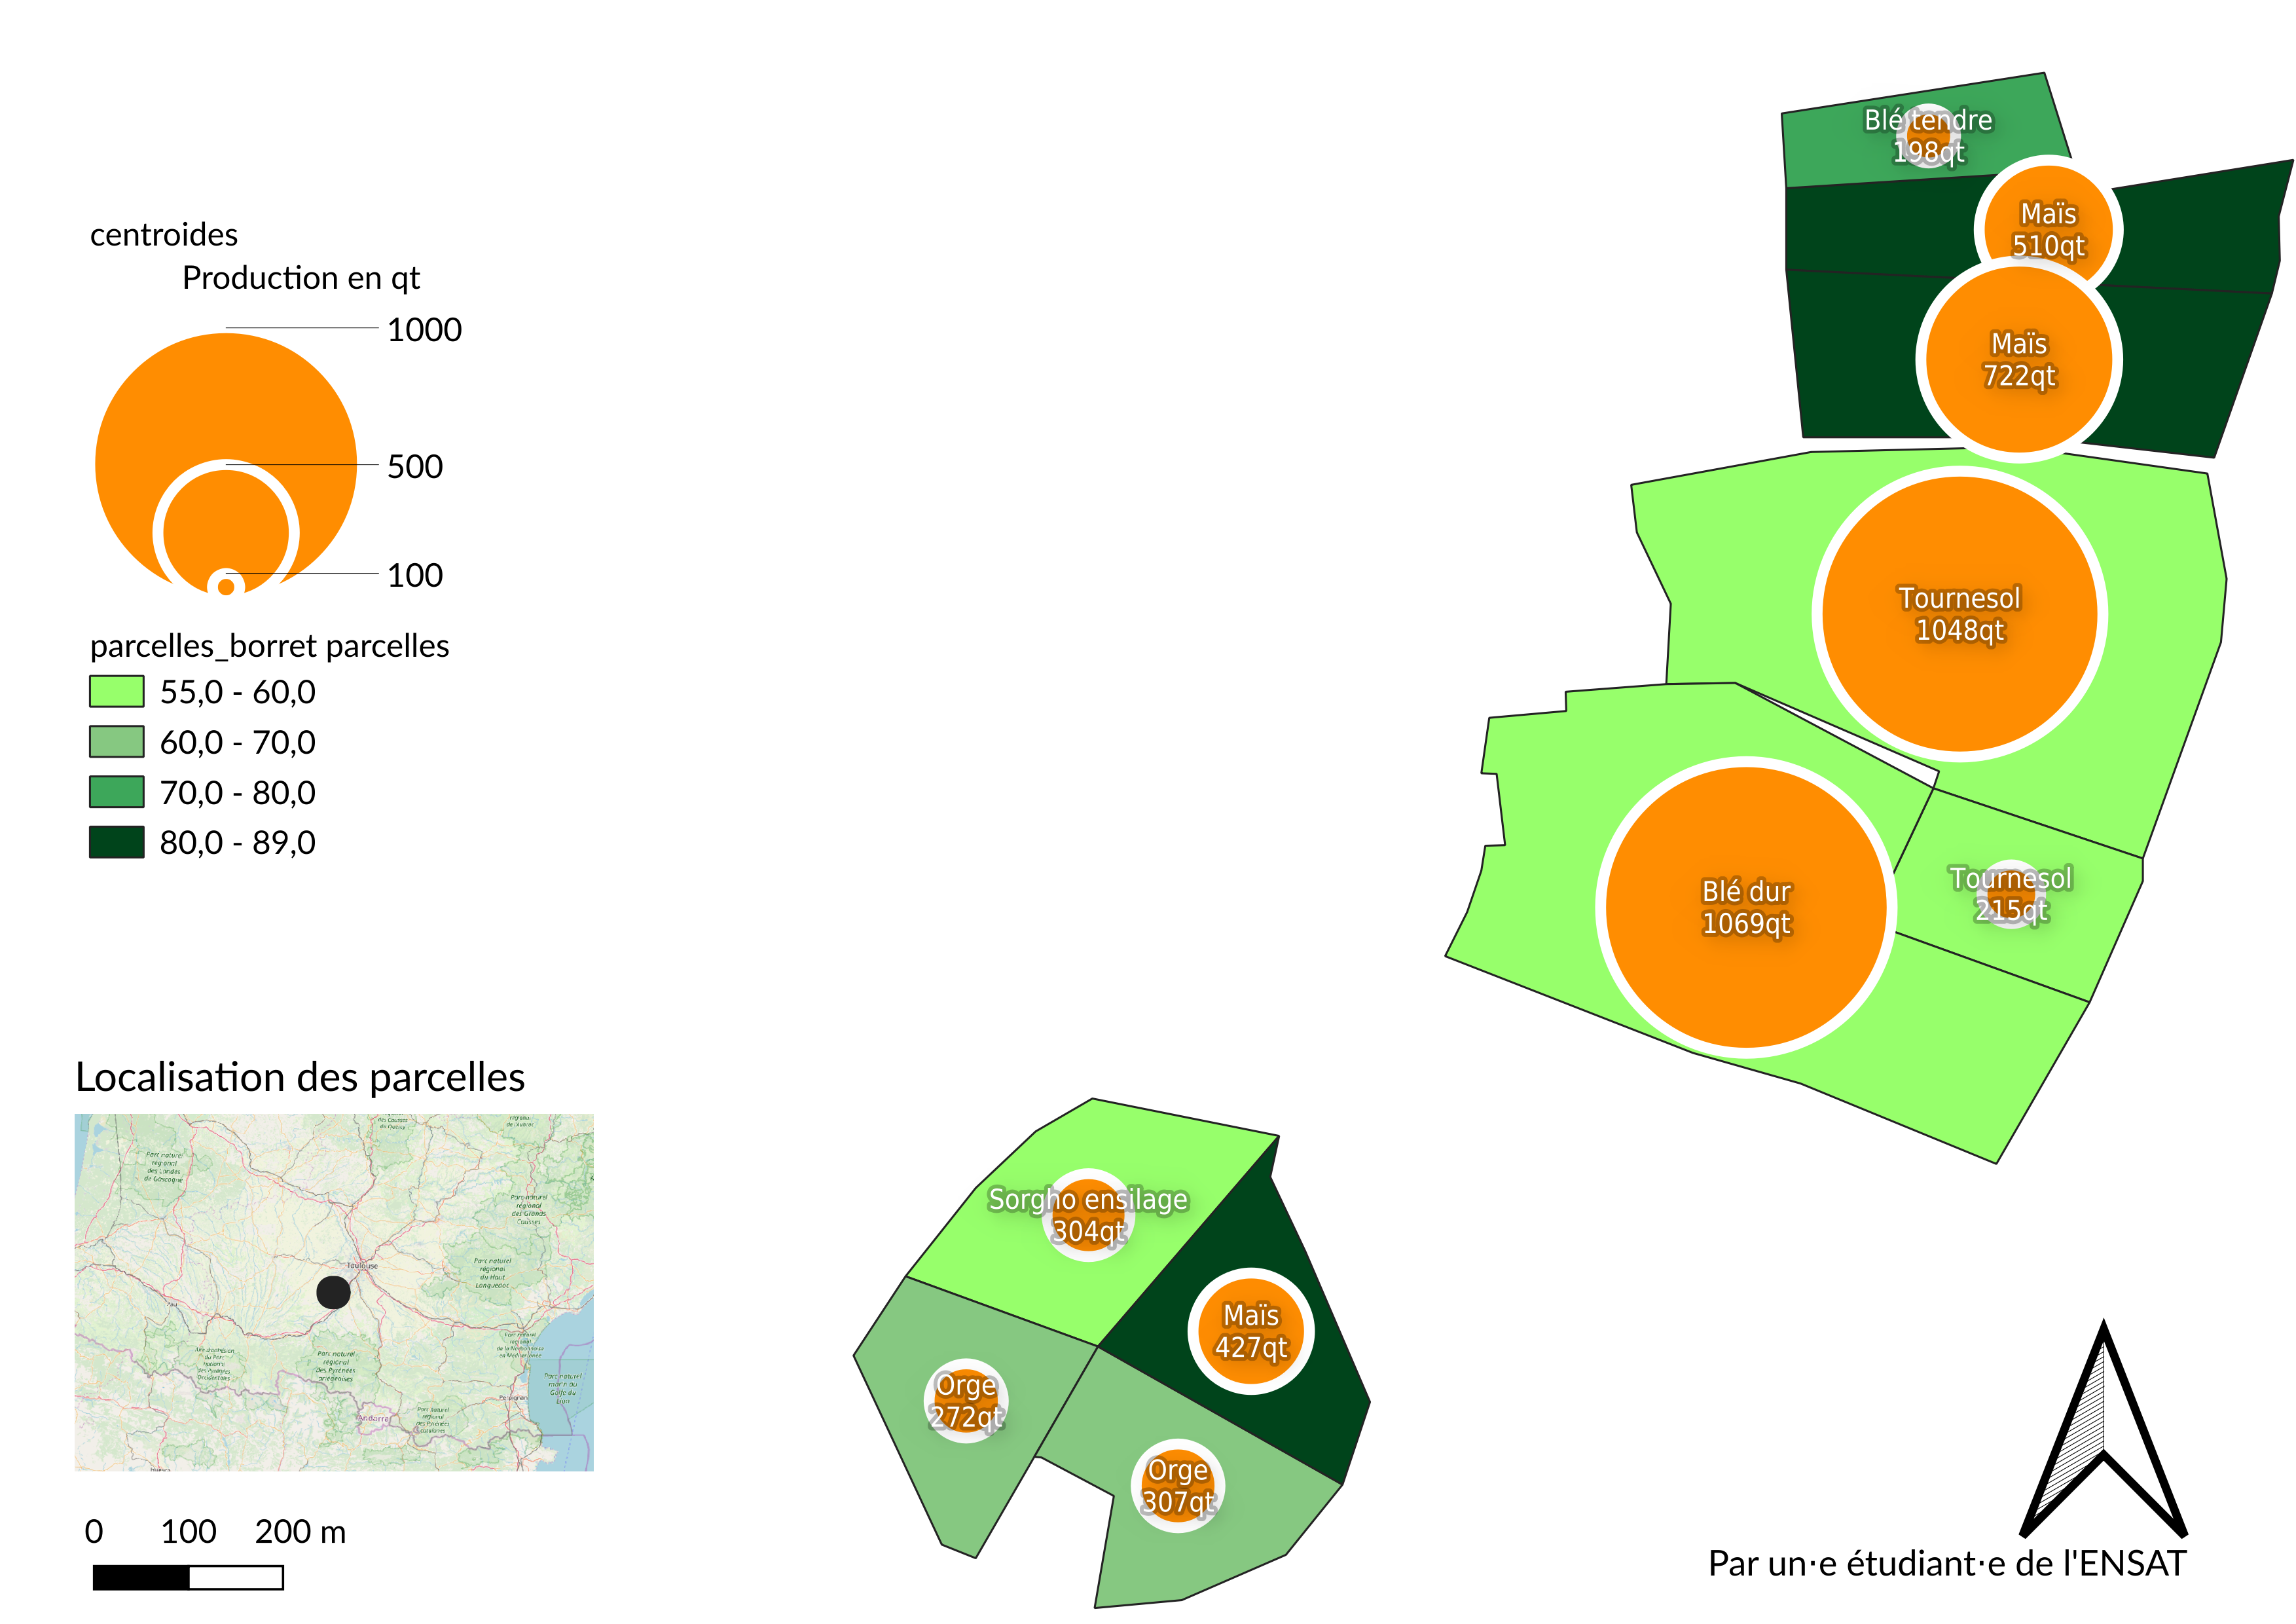
\includegraphics{figures/map_withloc.png}
\caption{Carte avec localisation de la zone d'étude en utilisant des
couches différentes}
\end{figure}

\hypertarget{guxe9nuxe9ration-dun-atlas}{%
\section{Génération d'un atlas}\label{guxe9nuxe9ration-dun-atlas}}

Un atlas permet de générer des cartes détaillées en utilisant un modèle
identique. Cela est par exemple utilisé pour faciliter le travail de
terrain en montrant précisément chaque parcelle qui sera étudiée in
situ.

L'objectif de l'atlas dans notre cas d'étude est de montrer pour chaque
parcelle sa production totale en qt et d'indiquer le type de culture.

Cliquer sur l'icône \texttt{Paramètres\ de\ l\textquotesingle{}atlas} du
menu du composeur d'impression Qgis, puis cocher dans la fenêtre en bas
à droite \texttt{Générer\ un\ atlas}.

Cliquer sur votre carte avec l'outil
\texttt{Sélectionner\textbackslash{}Déplacer\ un\ objet} et dans
\texttt{Propriété\ de\ l\textquotesingle{}objet} cocher
\texttt{Controlée\ par\ Atlas}.

La couche de couverture est la couche pour laquelle chaque entité sera
utilisée par QGIS pour générer chaque page de l'atlas. Nous choisirons
ici le polygone des parcelles.

Une fois l'atlas créé, sélectionner votre carte principale (et pas celle
de la localisation des parcelles), aller dans
\texttt{Propriétés\ des\ objets} et cocher la partie
\texttt{Contrôlé\ par\ l\textquotesingle{}atlas}. Vous pouvez désormais
demander à générer votre atlas en cliquant sur le bouton
\texttt{Aperçu\ de\ l\textquotesingle{}atlas}.

\begin{figure}
\centering
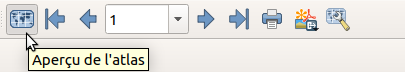
\includegraphics[width=\textwidth,height=0.625in]{figures/generate_atlas.png}
\caption{Aperçu de l'atlas}
\end{figure}

Pour ajouter des valeurs (textuelles ou numériques) en fonction de votre
parcelle (comme la production en qt), ajouter un champ texte (icône
texte sur la gauche), cocher la case \texttt{Rendu\ en\ html} puis
cliquer sur \texttt{Insérer\ une\ expression...}.

Ainsi, il ne sera plus obligatoire d'utiliser la fonction
\texttt{concat} car chaque variable sera mise entre crochets et entre
\%, comme par exemple :

\begin{verbatim}
En 2018, la parcelle n [% "id_parcelle" %] a produit  [% "prod_totale" %] qt de [% "assolement_2018_type" %]
\end{verbatim}

Votre atlas sera donc composé de 10 cartes, dont l'une sera du style :

\begin{figure}
\centering
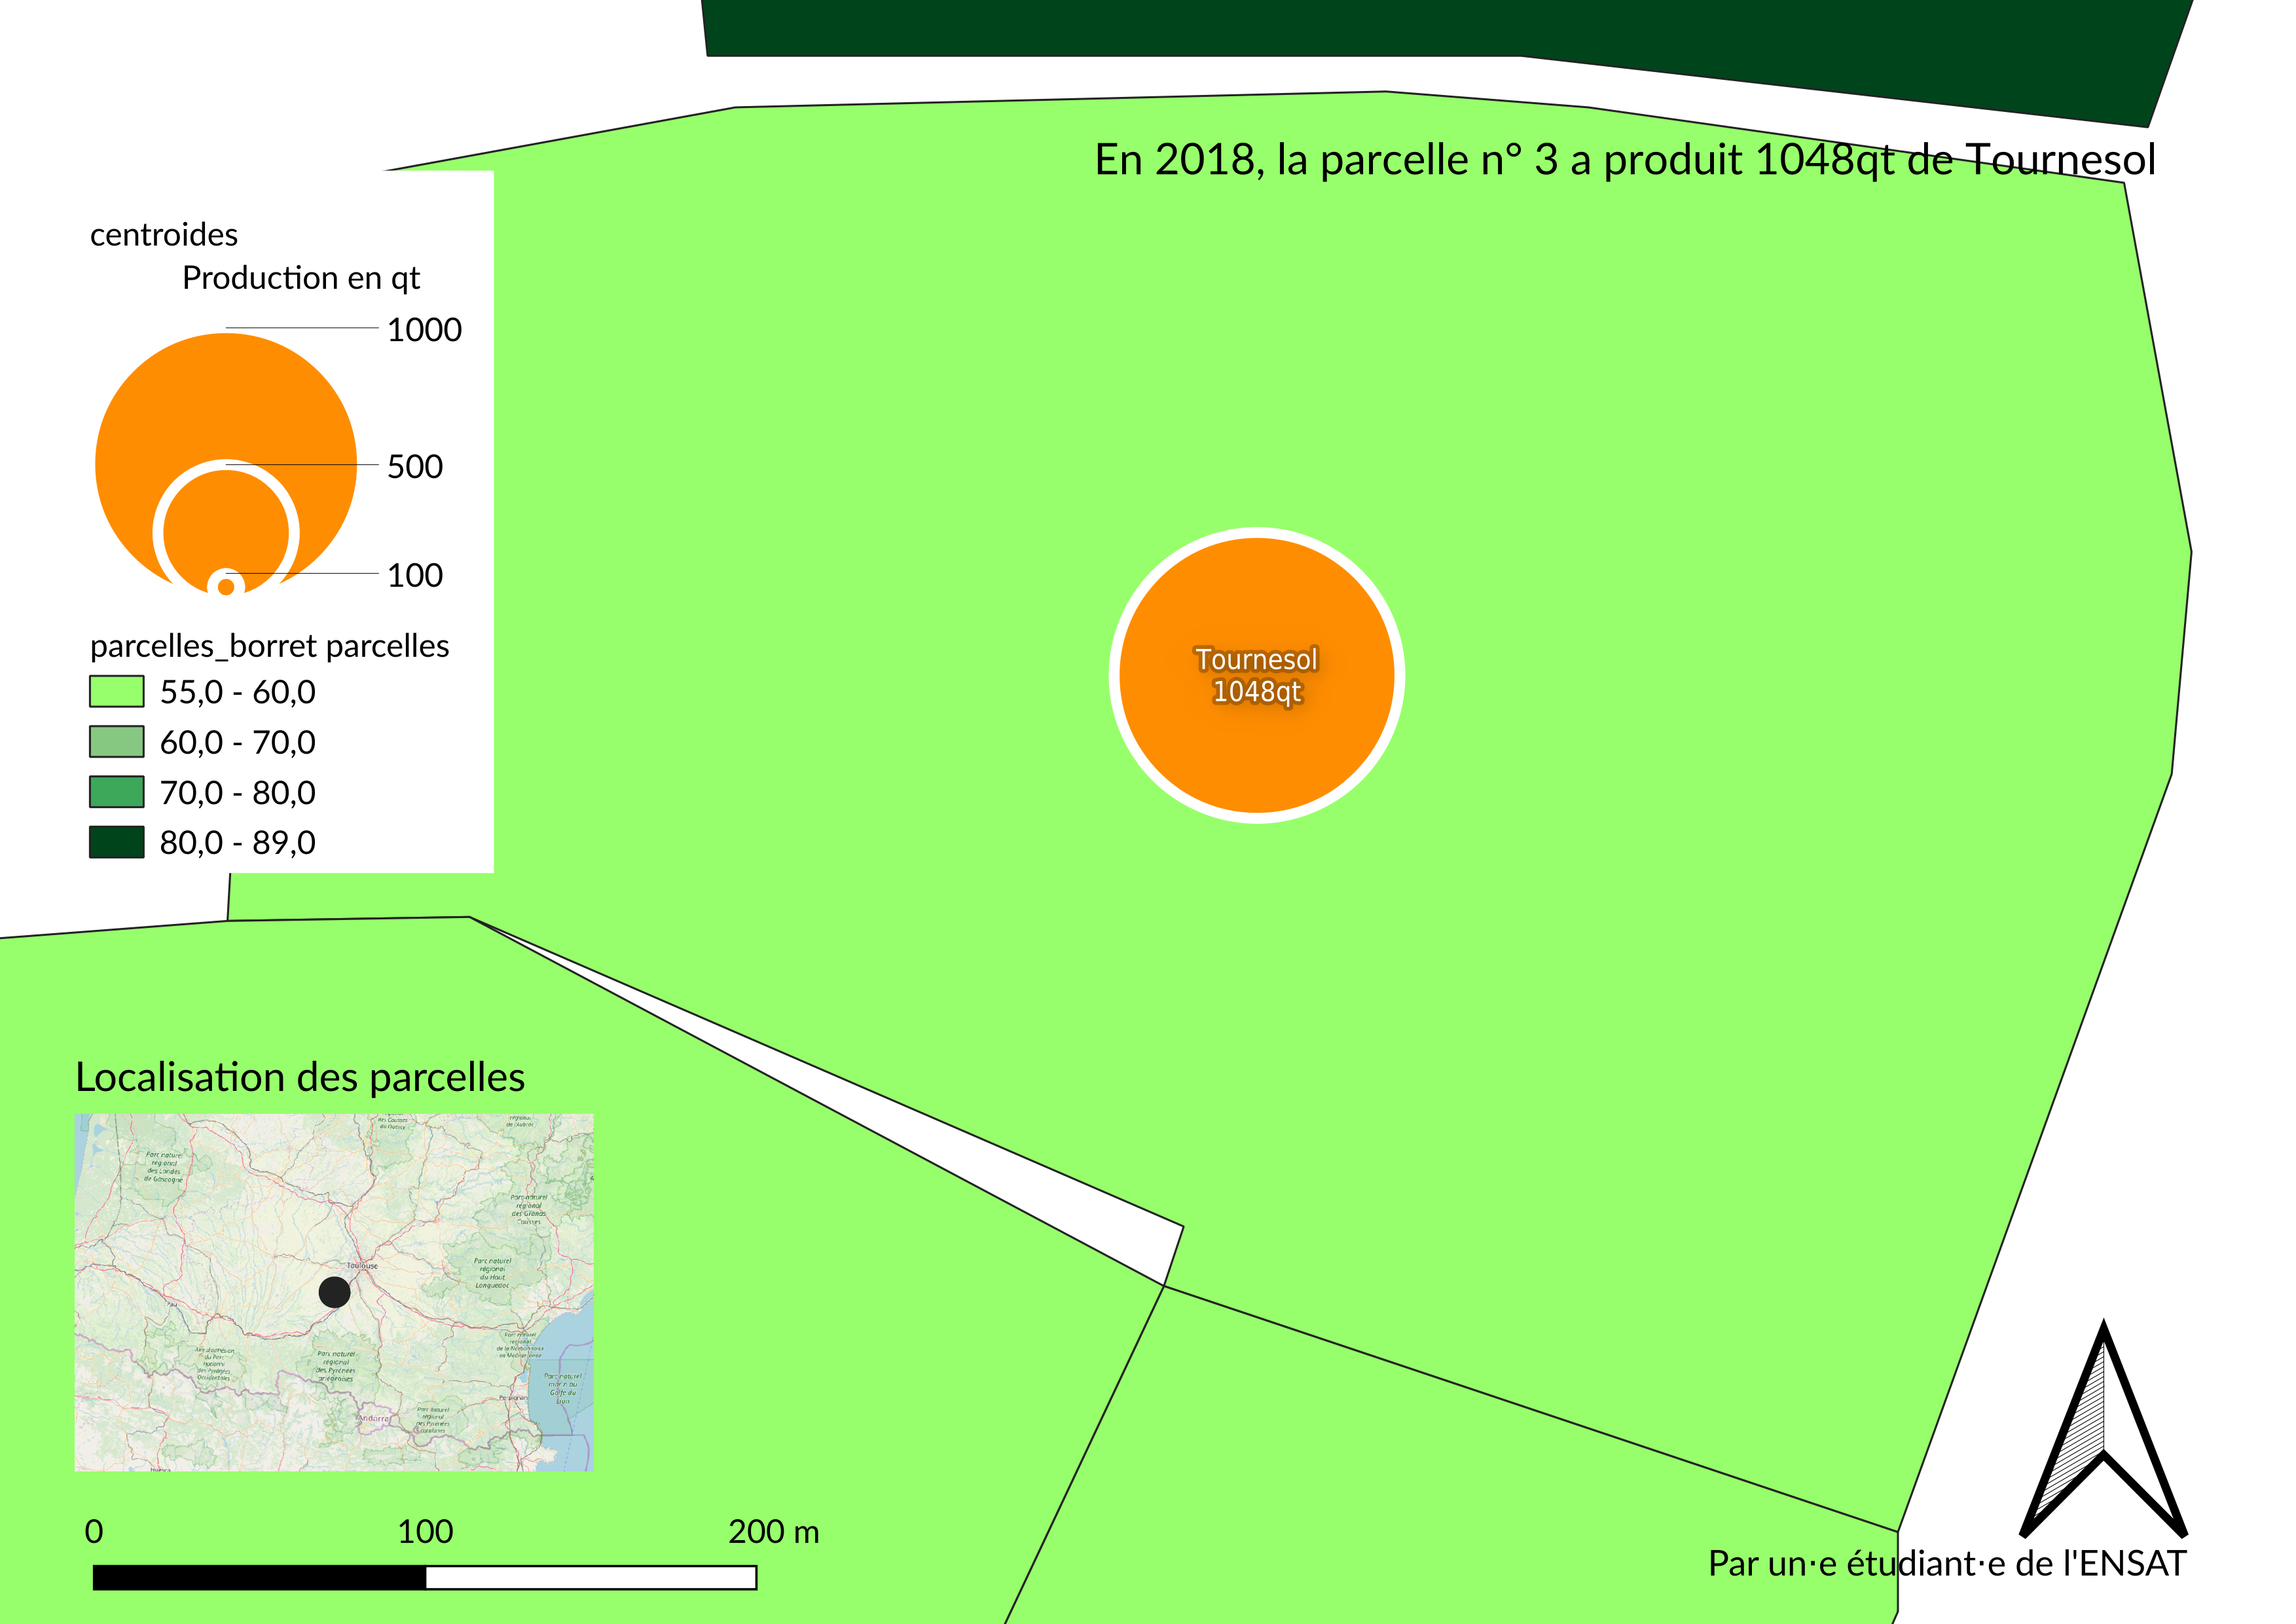
\includegraphics{figures/map_atlas.png}
\caption{Exemple de l'atlas de la parcelle n3}
\end{figure}
